\documentclass[aspectratio=169]{beamer}
\usepackage{minted}
\usepackage{listings}
\usetheme{veit}
\title{SCHEME: An Interpreter for Extended Lambda Calculus}
\subtitle{Gerald J. Sussman and Guy L. Steele Jr.}
\date{\today}
\author{Veit Heller}
\institute{Papers We Love Berlin}
\begin{document}
  \maketitle
  \begin{frame}{Agenda}
    \begin{itemize}
      \item Introduction and historical context
      \item Scheme primer
      \item The good stuff
      \item Let’s see some code!
      \item Implementation notes
    \end{itemize}
  \end{frame}
  \section{Introduction}
  \begin{frame}{The Paper}
    In 1975, a 21-year-old grad student named Guy Steele and his thesis
    advisor Gerald Sussman had something to show to the world: a little
    programming language called Scheme.
  \end{frame}
  \begin{frame}{The Paper}
    \begin{figure}
      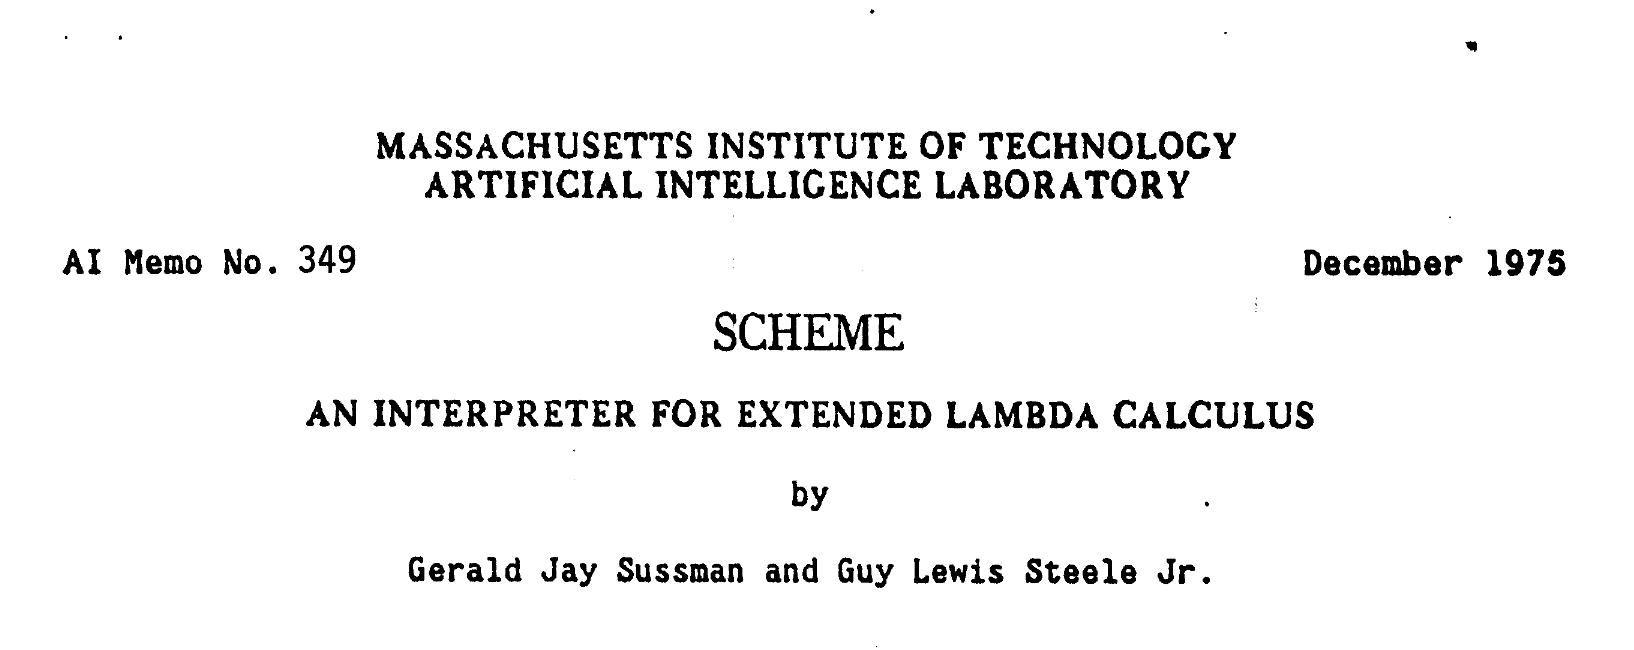
\includegraphics[width=\linewidth]{header.png}
      \caption{A wild paper appears.}
    \end{figure}
  \end{frame}
  \begin{frame}{The Paper}
    The paper has all the goods a hacker could wish for: a reference, cool code
    examples, and an implementation of Lisp in Lisp.
  \end{frame}
  \begin{frame}{The Name}
    The language was originally intended to be called SCHEMER, in reference
    to its ancestors PLANNER and CONNIVER.
  \end{frame}
  \section{Scheme: A primer}
  \begin{frame}[fragile]
    \frametitle{Scheme: A primer}
    In Scheme, we define functions using \texttt{define}—you might know it as
    \texttt{defn} or \texttt{defun} in other Lisps:

    \begin{listing}[H]
      \caption{Defining addition}
      \begin{minted}{scheme}
(define add
  (lambda (x y)
    (+ x y)))
      \end{minted}
    \end{listing}

    NB: I eschewed the all-caps notation, and I hope your eyes will thank me
    for it.
  \end{frame}
  \begin{frame}[fragile]
    \frametitle{Scheme: A primer}
    We can \texttt{quote} things using either the function or the abbreviation
    \texttt{'<thing>}.

    \begin{listing}[H]
      \caption{Using symbols as values}
      \begin{minted}{scheme}
; this will always return the symbol x
(define gimme-x (lambda () 'x))
      \end{minted}
    \end{listing}
  \end{frame}
  \begin{frame}[fragile]
    \frametitle{Scheme: A primer}
    There is also the somewhat idiosyncratic \texttt{labels}, which allows you
    to define local functions that can be called inside a context, and can call
    themselves and other local functions in that context. You might know it as
    \texttt{letrec*} from later Schemes, and as simply \texttt{let} in Common
    Lisp.
  \end{frame}
  \begin{frame}[fragile]
    \frametitle{Putting it all together}
    \begin{listing}[H]
      \caption{Let’s define something!}
      \begin{minted}{scheme}
; lets define cells!
(define cons-cell (lambda (contents)
    (labels ((the-cell
                (lambda (msg)
                  (if (eq msg 'contents) contents
                    (if (eq msg 'cell?) 'yes
                      (if (eq (car msg) '<-)
                        (block (aset 'contents (cadr msg))
                               the-cell)
                        (error '|Unrecognized Message - Cell|
                               msg
                               'wrng-type-arg)))))))
      the-cell)))
      \end{minted}
    \end{listing}
  \end{frame}
  \begin{frame}{And now?}
    There is more, though!
  \end{frame}
  \section{The good stuff}
  \begin{frame}[fragile]
    \frametitle{Continuations!}
    \begin{listing}[H]
      \caption{Jump around aka. “Sussman’s favorite style/Steele’s least favorite”}
      \begin{minted}{scheme}
(define sqrt (lambda (x epsilon)
  ((lambda (ans looptag)
    (catch returntag ; setup return label
      (progn
        (aset 'looptag (catch m m)) ; setup loop label
        (if (< (abs (- (* ans ans) x)) epsilon)
          (returntag ans) ; goto return label
          nil) ; not done yet
        (aset 'ans (/ (+ (/ x ans) ans) 2.0)) ; calculate step
        (looptag looptag)))) ; goto loop label
    1.0
    nil)))
      \end{minted}
    \end{listing}
  \end{frame}
  \begin{frame}{Wait, what?}
    Continuations effectively allow us to pause and resume computations, to
    pretend to call a function but instead moving between different interpreter
    states.
  \end{frame}
  \begin{frame}{Wait, what?}
    It’s pretty mind-bending at first and I understand if it’s a little much.

    \bigskip

    \small The paper is a bit harsh here: “Anyone who doesn’t understand how
    this manages to work probably should not attempt to use CATCH.”
  \end{frame}
  \begin{frame}{Multiprocessing}
    As if that wasn’t enough, we also have a multiprocessing story. We can
    create new processes using \texttt{create!process}, start them using
    \texttt{start!process}, stop them using \texttt{stop!process}, and
    synchronize using \texttt{evaluate!uninterruptibly}.
  \end{frame}
  \begin{frame}{Oof.}
    
\includegraphics[width=14cm]{reference_end.png}
  \end{frame}
  \section{Code Examples}
  \begin{frame}[fragile]
    \frametitle{Continuations, yet again!}
    \begin{listing}[H]
      \caption{Factorial, but the computation happens in continuations.}
      \begin{minted}{scheme}
(define fact (lambda (number continuation)
  (if (= number 0)
    (continuation 1)
    (fact (- number 1)
          (lambda (a) (continuation (* number a)))))))

; simple computation
(fact 5 (lambda (x) x))

; computation, but we log each step
(fact 5 (lambda (x) (block (print x) x)))
      \end{minted}
    \end{listing}
  \end{frame}
  \begin{frame}{Multiprocessing}
    Consider you have two functions, and you want to run them in parallel,
    stopping whenever the first one terminates, and returning its result.

    \bigskip

    The authors call this “A Useless Multiprocessing Example”.
  \end{frame}
  \begin{frame}[fragile]
    \frametitle{Multiprocessing}
    \begin{listing}[H]
      \caption{Dont!Shout!At!Me}
      \begin{minted}{scheme}
(define try!two!things!in!parallel (lambda (f1 f2)
  (catch c
    ((lambda (p1 p2)
      ((lambda (f1 f2)
        ; ensures both fs get started atomically
        (evaluate!uninterruptibly
          (block (aset 'p1 (create!process '(f1)))
                 (aset 'p2 (create!process '(f2)))
                 (start!process p1)
                 (start!process p2)
                 (stop!process **process**)))) ; stop yourself
          ; what are f1 and f2?
          ))
      nil nil))))
      \end{minted}
    \end{listing}
  \end{frame}
  \begin{frame}[fragile]
    \frametitle{Multiprocessing}
    \begin{listing}[H]
      \caption{The magic bits}
      \begin{minted}{scheme}
; f1 = 
(lambda ()
  ; stop the other process and return
  ((lambda (value)
    (evaluate!uninterruptibly
      (block (stop!process p2) (c value))))
   (f1))) ; do our thing
; f2 =
(lambda ()
  ((lambda (value)
    (evaluate!uninterruptibly
      (block (stop!process p1) (c value))))
   (f2)))
      \end{minted}
    \end{listing}
  \end{frame}
  \begin{frame}[fragile]
    \frametitle{Pattern matching!}
    Let’s consider a simple pattern matching function.
    \begin{listing}[H]
      \caption{A simple pattern matcher.}
      \begin{minted}{scheme}
; ! = zero or more things (.* in regex)
; ? = any single thing (. in regex)
; anything else = itself

(match '(A !B ?C ?C !B !E)
       '(A X Y Q Q X Y Z Z X Y Q Q X Y R))
      \end{minted}
    \end{listing}
  \end{frame}
  \begin{frame}{Pattern matching!}
    Instead of just returning the match groups, however, we return the match
    groups and a continuation that gives us backtracking and will return
    alternative matches, Prolog-style.

    \bigskip

    How would we implement this?
  \end{frame}
  \begin{frame}{Pattern matching!}
    \begin{figure}
      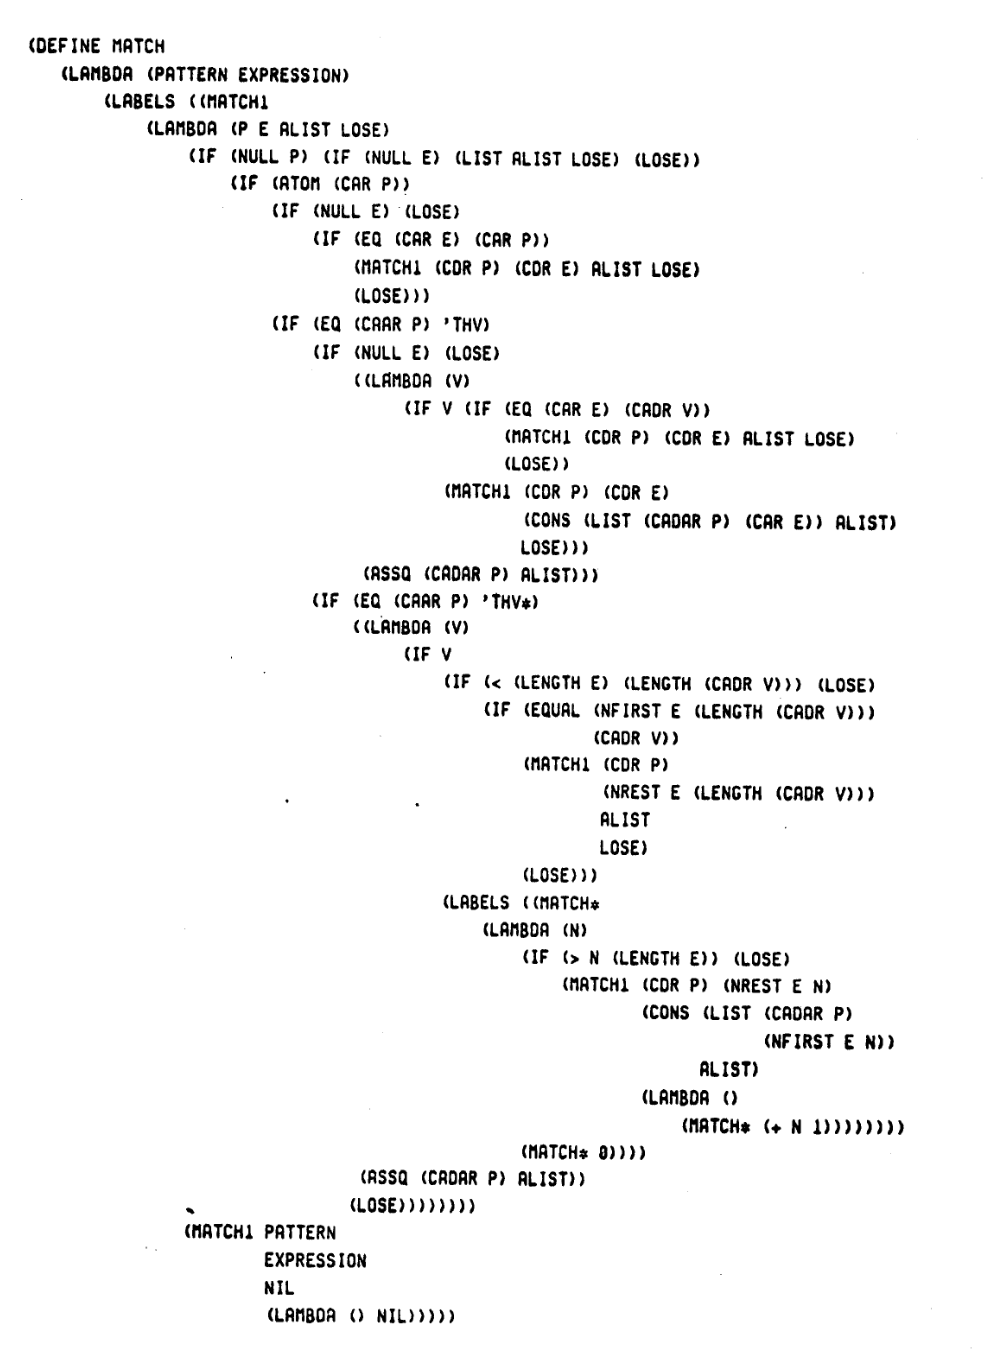
\includegraphics[height=7cm]{match.png}
      \caption{A simple solution to a simple problem.}
    \end{figure}
  \end{frame}
  \begin{frame}{Examples I wish I would have had time for}
    If you have the time to study the code examples, keep your eyes peeled
    for the definition of the \texttt{do} macro and the \texttt{samefringe}
    problem.
  \end{frame}
  \section{Implementation Notes}
  \begin{frame}{The interpreter}
    The design of the interpreter is deceivingly straightforward.
  \end{frame}
  \begin{frame}{The interpreter}
    It is
    \begin{itemize}
      \item lexically scoped,
      \item based on continuations and “clinks”,
      \item built on top of MacLISP (all of MacLISP is available as a primitive),
      \item not purely functional, and
      \item concurrent (but not parallel).
    \end{itemize}
  \end{frame}
  \begin{frame}{The implementation}
    \begin{figure}
      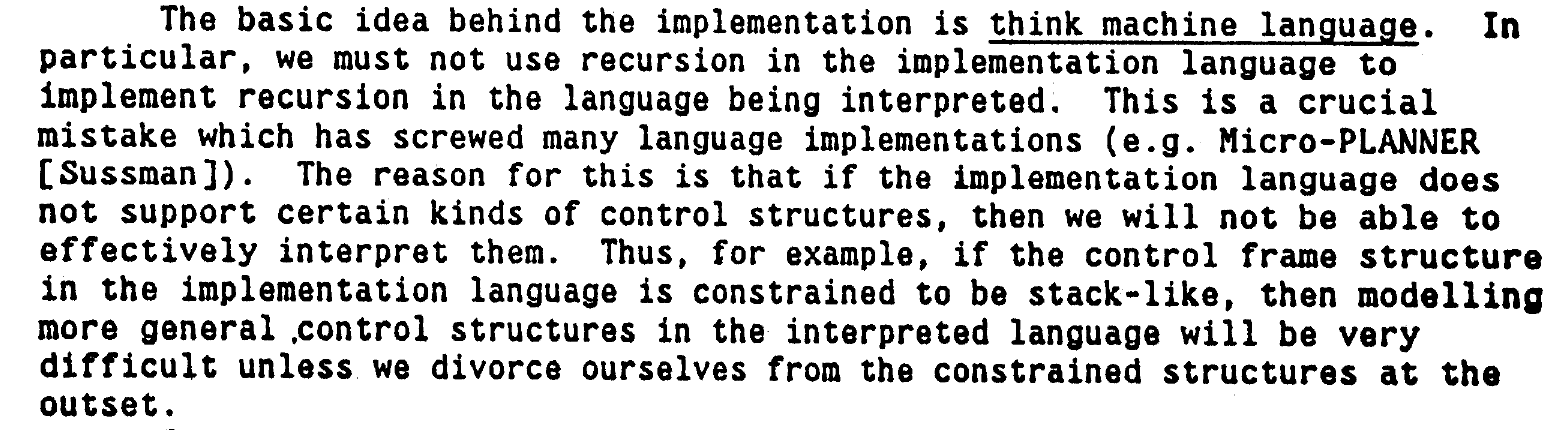
\includegraphics[width=14cm]{implementation.png}
    \end{figure}
  \end{frame}
  \begin{frame}{The implementation}
    It is striking to me how readable the implementation is.
  \end{frame}
  \begin{frame}{The implementation}
    If you tried to read the implementation but gave up, here are a few pointers:

    \begin{itemize}
      \item Start in the evaluation loop.
      \item Find out how components work.
        \begin{itemize}
          \item “Where do clinks pass through?”
          \item “What happens when I call \texttt{catch}?”
        \end{itemize}
      \item Trace a program (if you must).
    \end{itemize}
  \end{frame}
  \begin{frame}[fragile]
    \frametitle{The implementation}
    Let’s look at a primitive: \texttt{if}.

    \begin{listing}[H]
      \caption{The internals of \texttt{if}.}
      \begin{minted}{scheme}
(defun if ()
  (saveup 'if1) ; we will go there next
  (setq **exp** (cadr **exp**) ; first eval the condition
        **pc** 'aeval))

(defun if1 ()
  (cond
    (**val** ; the condition was true, take then
      (setq **exp** (caddr **exp**))
     t ; otherwise take else
      (setq **exp** (cadddr **exp**))))
  (setq **pc** 'aeval))
      \end{minted}
    \end{listing}
  \end{frame}
  \begin{frame}{Amen}
    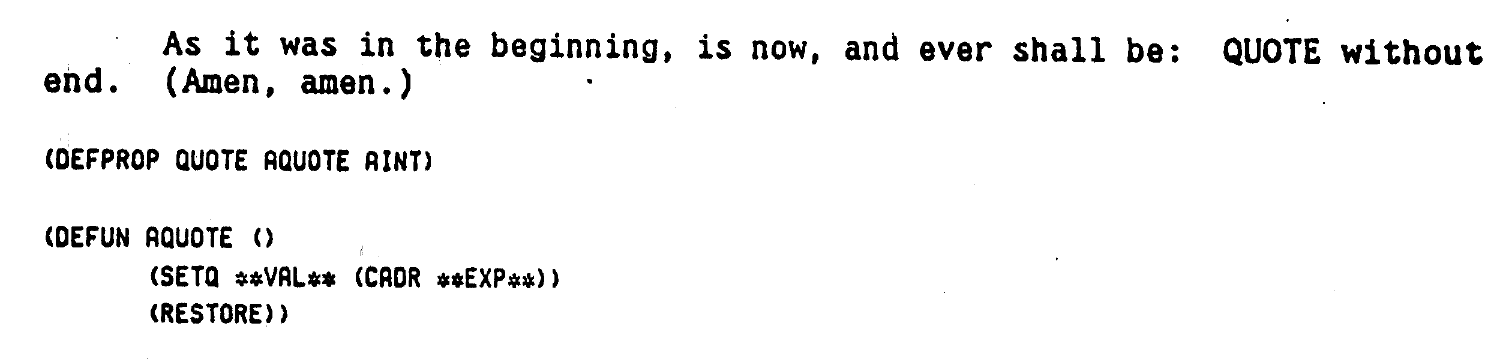
\includegraphics[width=14cm]{amen.png}
  \end{frame}
  \begin{frame}{That’s it?}
    Cool, so that’s all there is to it?
  \end{frame}
  \begin{frame}{That’s it?}
    Let’s talk about the multiprocess primitives really quick.
  \end{frame}
  \begin{frame}{Implementing threads}
    This is what we need to do:

    \begin{itemize}
      \item Creating a process creates new registers and sets up a new interpreter
      \item Starting a process puts it in the process queue.
      \item Stopping a process removes it from the process queue and terminates it if it is the current process.
      \item Evaluating uninterruptibly means binding a flag to \texttt{nil} that tells the interpret er not to swap processes.
      \item Then we need to build a magical scheduler that swaps process in the queue once in a while.
    \end{itemize}

    Ta-dah!
  \end{frame}
  \begin{frame}{Implementing continuations}
    What about continuations?

    \begin{itemize}
      \item \texttt{catch} tells the evaluator to switch the clink.
      \item Then we need to know how and when to switch these out in the main loop (hint: look at \texttt{evlis}).
      \item Swapping process becomes almost equivalent to swapping continuations!
    \end{itemize}

    Ta-dah!
  \end{frame}
  \begin{frame}{Implementing macros}
    
\includegraphics[width=14cm]{beasties.png}
  \end{frame}
  \begin{frame}{Fin}
    
\includegraphics[width=14cm]{interpreter_end.png}
  \end{frame}
  \begin{frame}{References}
    \begin{itemize}
      \item Gerald Jay Sussman and Guy L. Steele, Jr.: Scheme—An Interpreter for Extended Lambda Calculus
      \item Guy L. Steele, Jr.: Rabbit—A Compiler for Scheme
      \item John C. Reynolds: The Discoveries of Continuations
      \item Irene Greif and Carl Hewitt: Actor Semantics of PLANNER-73
      \item These slides: \texttt{https://github.com/hellerve/talks}
      \item The \texttt{match} function on my blog: \texttt{blog.veitheller.de/Pattern\_Matching,\_A\_Thing\_Of\_The\_Past.html}
      \item A series of blog posts on Scheme macros: \texttt{https://blog.veitheller.de/scheme-macros}
    \end{itemize}
  \end{frame}
  \begin{frame}{The End}
    \Huge Thank you!
    \linebreak
    \linebreak
    \linebreak
    \small Questions?
    \linebreak
    \linebreak
    \tiny Slides at \texttt{https://github.com/hellerve/talks}
  \end{frame}
\end{document}
